%!root = ../main.tex
% 极端气候定义、风险偏好=>风险厌恶程度、家财险定义
\chapter{引言}
\section{研究背景与意义}
% 背景、政策、数据
全球气候变化正在导致极端天气事件的频率和强度显著增加,如图\ref{fig:swissre}所示。随着气候变化及其诱发的自然灾害对我国的影响日益加剧,人民的生活安全和财产保障面临前所未有的挑战。应对气候变化是中国可持续发展的内在要求,也是中国积极参与全球治理、推动构建人类命运共同体的重要体现。党的二十大报告指出,“尊重自然、顺应自然、保护自然,是全面建设社会主义现代化国家的内在要求”,要“提高防灾减灾救灾和重大突发公共事件处置保障能力,加强国家区域应急力量建设”。中国作为一个自然灾害频发的国家,面临的自然灾害类型多样,包括但不限于洪涝、台风、干旱、风雹、低温冷冻和雪灾等。据2023年的统计数据显示,全年各种自然灾害共导致9544.4万人次不同程度受灾,直接经济损失高达3454.5亿元,部分极端天气事件如表\ref{tab:weather}所示。面对逐渐增大的气候变化风险,2023年10月24日,我国政府宣布增发2023年国债,总额达1万亿元,专项用于灾后恢复重建工作和提升国家防灾减灾的整体能力\footnote{资料来源:新华社,\url{https://www.gov.cn/yaowen/liebiao/202310/content_6911405.htm}}。这一战略决策不仅体现了政府对气候变化引发的灾害风险的高度警觉,也彰显了加强防灾减灾工作的紧迫性和重要性。

\begin{figure}[htbp]
    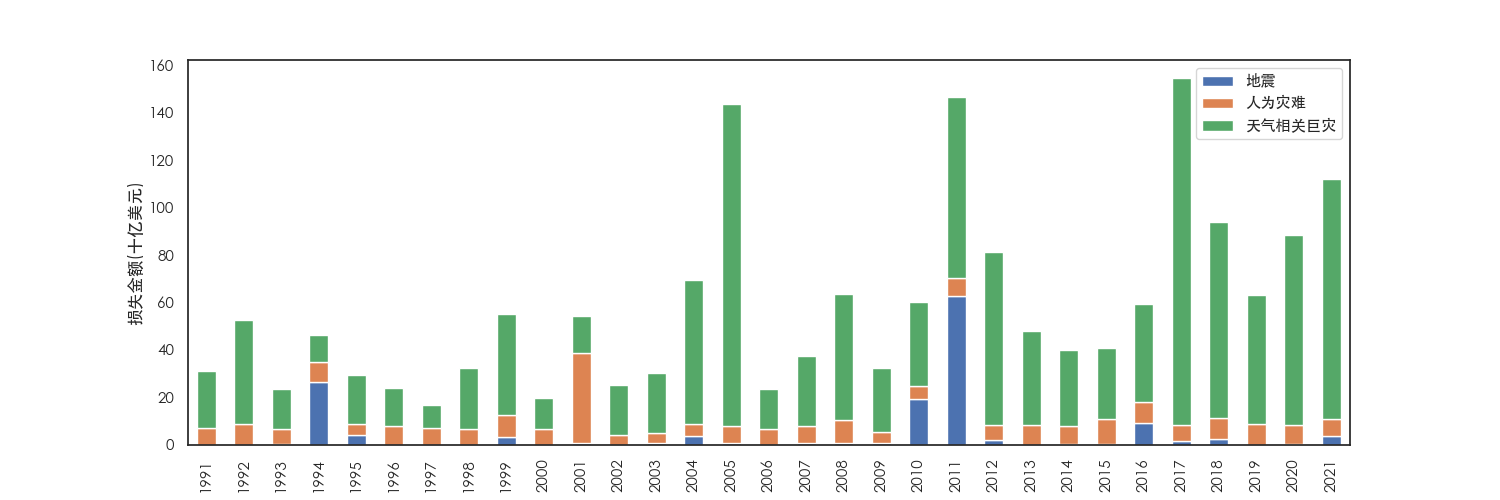
\includegraphics[width=\linewidth]{img/disaster.png}
    \caption{全球自然灾害带来的损失(单位:十亿美元)}\label{fig:swissre}
    \qquad \zihao{5} 资料来源:SwissRe, Sigma, 2024年第1期
\end{figure}

\begin{table}[h]
    \renewcommand{\arraystretch}{1.5}
    {\centering
    \caption{2023年我国部分极端天气事件}\label{tab:weather}
    \begin{tabular}{cccc}
        \toprule
        \textbf{日期} & \textbf{事件类型} & \textbf{影响地区} & \textbf{直接经济损失金额} \\
        \midrule
        1月13日-16日& 寒潮            & 福建、江西、云南      & 2.79亿元            \\
        3月11日–14日& 暴雪            & 河南            & 3.5亿元             \\
        4月初& 风雹            & 湖南、贵州、江西      & 16亿元              \\
        4月21日-24日& 低温冷冻和雪灾       & 山西、甘肃等11省     & 13.6亿元            \\
        4月下旬& 洪涝            & 湖南、湖北、福建      & 6.2亿元             \\
        5月6日-8日& 低温冷冻和雪灾       & 云南、新疆等9省      & 10.3亿元            \\
        5月初& 大风、冰雹         & 河北            & 13.5亿元            \\
        7月28日-31日& 超强台风“杜苏芮”     & 福建、浙江、安徽      & 147.4亿元           \\
        7月18日–20日& 风雹            & 内蒙古、山西        & 14亿元              \\
        8月初& 强降雨           & 黑龙江、吉林        & 170.9亿元           \\
        8月11日-15日& 台风“卡努”        & 辽宁、黑龙江        & 9.2亿元             \\
        10月19日-20日& 台风“三巴”        & 广东、广西、海南      & 58.2亿元            \\
        10月上中旬& 洪涝            & 湖北、四川、贵州      & 4.6亿元             \\
        \bottomrule
    \end{tabular}}
    \par\qquad \zihao{5} 资料来源:应急管理部,\url{http://www.mem.gov.cn/gk/tjsj/}
\end{table}

在这一宏观背景下,探讨极端天气是否增大了人们的风险厌恶程度及其具体表现形式,对于了解风险承担者在风险冲击下风险意识的变化,具有重要意义。该研究不仅能够丰富我们对气候变化社会经济影响的理解,还能为制定更为科学、前瞻性的风险管理策略提供理论依据和实践指导。通过深入分析气候变化如何塑造个体和群体的风险认知与决策行为,我们可以更有效地实施风险管理措施,这不仅有助于提高社会的适应能力和韧性,也是推动构建和谐、稳定、可持续发展社会的关键步骤。

随着极端气候事件的频繁发生,人们对自身及财产的安全日益关切。在灾害面前,家庭往往是首当其冲的受害者。但与企业相比,个人和家庭对这些潜在风险的反应可能更为复杂。家庭是否会通过购买家财险来缓解财产损失,以及他们在灾害发生后是否更加倾向于购买保险,对这一问题的观察与分析,有助于加强对灾害冲击-反应的理解。

然而,极端天气下人们对自身及财产安全的关切是否能够持续转化为对保险的需求,尤其是在家庭层面,却是一个相对较少被深入研究的领域。以往研究的对象包括气候变化对企业财产险\citep{杨娜娜2019自然灾害与企业现金持有}或健康险\citep{赵强2021空气污染对商业健康保险需求的影响}需求的影响,以及雾霾天气对健康险需求的影响\citep{2018Something}等,但是对于家庭财产保险的定量研究却相对较少。本研究的选题来源于对这一领域的关注,探讨了极端天气极端冲击对家财险需求的影响,丰富了极端天气冲击-反应的研究文献。

作为风险管理的手段之一,我国家财险市场的发展始于1980年,是当时中国人民保险公司的基础险种之一。1980年,全国范围内有34200户家庭购买了中国人保的家财险,保险金额为5232万元,保费仅为7万元,仅占国内产险保费总额的0.02\%。到了1989年,全国家财险(包括储蓄性两全险)的投保户数增至76,910,000户,保险金额达1974亿元,保费收入为3.2亿元,占产险保费总额的4.4\%。可以说,我国财产保险的早期发展同时也是家庭财产保险发展的过程\citep{黄英君2008论我国产险公司分散性业务营销模式的创新},塑造了消费者对财产险最早的认知。之后家财险市场发展较为稳定,虽然2022年家财险以67.22\%的增长率成为了保费增速最快的财产险险种,保费达到164亿,但规模占比还不高,2022年末家财险保费收入占财产险保费收入的比例不足1.3\%\footnote{资料来源:中国消费者报,\url{https://www.ccn.com.cn/Content/2023/08-22/1307315925.html}},家财险市场在未来还有很大发展空间。
\begin{figure}[htbp]
    {\centering
        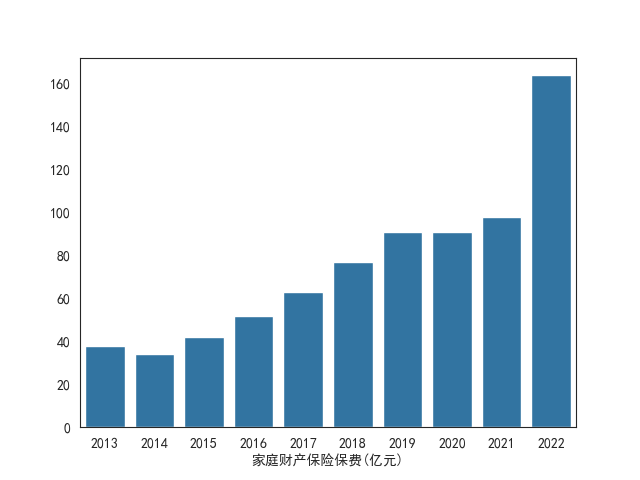
\includegraphics[width=0.8\linewidth]{img/家庭财产保险保费.png}\par }
    \caption{家庭财产保险保费收入}
    \qquad \zihao{5} 资料来源:国家统计局网站,\url{https://data.stats.gov.cn/easyquery.htm?cn=C01&zb=A0L0E01&sj=2022}
\end{figure}


本文将通过深入研究极端天气对家财险需求的影响,探索个人家庭在面对气候变化时的风险管理行为的特征,为政策制定提供更全面的支持。本研究的意义不仅仅停留在学术层面,更涉及到社会和经济发展的多个方面:

首先,从保险行业的角度来看,本研究能够帮助保险公司更好地理解极端天气事件对家财险市场需求的影响。通过分析家庭在面对气候变化时的风险管理行为,保险公司可以更深入了解市场需求,从而优化产品设计、定价策略和营销方案,增强行业的稳定性和可持续发展能力。

其次,从社会科学的角度来看,本研究丰富了人们在面对自然灾害时的行为和决策模式方面的证据。通过分析家庭在极端天气事件前后的保险购买行为,可以揭示人们的风险感知、风险态度和风险应对策略,为心理学、社会学和行为经济学等领域提供丰富的研究素材。这对于理解和预测人们在危机情境下的行为反应,以及设计有效的危机干预和应对措施具有重要意义。

最后,从可持续发展的角度来看,本研究有助于推动社会对气候变化风险的认识和应对。通过揭示保险在气候变化适应和减缓中的作用,可以增强公众的风险意识,提高对保险作为风险管理工具的认识和接受度。这不仅有助于促进保险市场的健康发展,还能够推动形成一种更加理性、科学的社会文化氛围,鼓励个人和社会共同参与到气候变化的应对中来,共同构建一个更加安全、可持续的未来。

\section{研究框架}
根据ETCCDI的定义,极端天气冲击可以分为两大类:极端降水和极端温度。本文选取极端降水作为准自然实验,通过构造双重差分模型,考察发生极端降水后,家财险投保是否有显著提升,以此探究极端天气事件冲击下家庭的行为反应。

本文的结构安排如下:第\ref{chap:2}章是文献综述与研究假说。本章梳理关于气候变化对保险需求影响的研究,探讨风险感知的相关理论及其影响因素,分析自然灾害如何影响个人和企业的风险感知,以及这些变化如何反映在保险购买行为上。在文献综述的基础上,提出本研究的三个主要假说。这些假说的提出基于现有文献的不足和本研究的独特视角,旨在研究关于家庭财产保险需求对极端天气事件反应。

第\ref{chap:3}章研究设计,将详细介绍本研究所采用的方法论框架、数据来源及处理方式、以及模型设定和变量定义。首先,界定极端天气事件的范围,并根据ETCCDI标准选取极端降水作为研究重点。接着,将描述样本选择的过程,包括数据的时间和空间范围,以及数据清理的具体步骤。最后,详细阐述所采用的计量经济模型,包括基础的回归分析和双重差分(DID)方法,并解释模型中各变量的经济含义及其预期的作用。

第\ref{chap:4}章实证分析,对实证结果进行分析讨论。本章首先展示描述性统计数据,以揭示样本的基本特征。随后,报告回归分析的结果,包括基础回归和DID回归模型的估计结果,以及对模型稳健性的检验。此外,我们还将探讨极端天气事件对保险赔付和续约行为的影响,通过Logit回归分析来深入理解居民和保险公司在灾害后的行为变化。

第\ref{chap:4.1}章主要是扩展问题的实证结果,主要讨论地理位置、保单购买时间、保险标的价值和城乡环境等不同时,极端天气对家庭购买家财险的差异,进一步加强本文基本问题的逻辑性。

第\ref{chap:5}章总结本研究的主要发现,并讨论其对保险业和政策制定的潜在影响。我们将回顾研究假设的验证情况,探讨极端天气事件对家庭风险感知和保险需求的影响机制,并提出未来研究的可能方向,并就如何提高家庭财产保险市场的适应性和效率提出建议。
\section{研究创新与不足}
本文的创新点主要体现在以下几个方面:

第一,本文以家庭财产保险购买为研究对象,讨论了极端天气冲击的影响。已有文献大多以企业的反应为研究对象\citep{0Do},,针对个人反应的研究也以健康险\citep{赵强2021空气污染对商业健康保险需求的影响}、农险\citep{胡新艳2021气候变化}为主,对家庭和持续气候变化的关注较少,本文研究扩展了相关文献,为家庭财产保险需求的研究提供了新的视角。

第二,本文探究了极端天气事件冲击下,灾区和非灾区家庭财产保险需求的差异,并进一步分析了地区异质性和时间异质性,为保险公司开发相关产品,以及监管机构制定相关政策提供了参考,具有一定的政策借鉴意义。

尽管本研究取得了一定的成果,但仍存在一些局限性。首先,本研究主要关注了极端降水事件对家财险需求的影响,未来研究可以扩展到其他类型的极端天气事件。其次,本研究的数据来源于特定保险公司,尽管数据量很大,但仍可能存在样本选择偏差。未来的研究可以考虑使用更广泛的数据集,以增强研究结果的普遍性。

\chapter{文献综述与研究假说}\label{chap:2}
\section{文献综述}

本文主要从两个角度梳理国内外相关文献:一是自然灾害对个体风险管理行为的影响,二是气候变化对不同类型保险需求的影响。

\subsection{自然灾害对个体风险管理行为的影响}\label{sec:disaster}

从认知的角度看,自然灾害的经历会直接影响个体的风险感知。自然灾害改变了个体对背景风险的感知,使他们认为未来再次发生灾害的可能性增加\citep{dillenberger2015history,ZGRK202210006},因此经历过洪水或地震的个体往往会展现出更多的风险规避行为\citep{cameron2015risk,cassar2017trust}。这一现象符合心理学中的获得性启发理论\citep{tversky1973availability,0Do},即人们倾向于依赖最容易回忆起的信息来做出判断,因而容易高估或低估事件发生的概率。此外,灾难经历还可能导致回忆放大效应\citep{heir2009longitudinal,cheong2022natural},使得个体在悲观预期下触发自我保护机制,进而规避风险个体对过去经历的威胁强度回忆得更加严重\citep{dillenberger2015history},从而影响到他们的心理健康和应对行为。例如,汶川地震后,公众的风险感知显著增强,这不仅体现在对当前安全的担忧上,也体现在对未来可能发生的类似灾害的预期中\citep{李华强2009突发性灾害中的公众风险感知与应急管理,贾建民2008汶川地震重灾区与非重灾区民众风险感知对比分析}。

自然灾害的发生及其损失具有或然性,个体面对着巨灾冲击未来收入的不确定性,因此巨灾除了通过影响风险感知外,也可能通过财富效应冲击个体风险管理行为\citep{田玲2009中国财产保险业巨灾损失赔付能力实证研究}。例如位于台风路径上的企业倾向于持有更多现金\citep{0Do,杨娜娜2019自然灾害与企业现金持有}或调整债务结构\citep{shao2024typhoons}以规避融资约束、管理流动性以应对飓风风险带来的不确定性,平均而言飓风发生后邻近公司现金持有量会增加1.1\%,随着时间的推移现金持有量逐渐回到了飓风前的水平\citep{0Do}。
这一现象也在家庭层面得到了验证,例如地震后家庭财产结构的变化,家庭会减少对高风险金融资产的投资\citep{于也雯0财产和生命双重风险约束下的家庭资产选择,liu2022effect}、倾向于购买一些家财险,并减少购买彩票的概率\citep{章元0地震冲击对风险偏好的影响}。

除了直接的冲击和损失会影响人们的风险管理措施,有关灾难的间接风险信息也会对人们的风险决策有影响\citep{said2015risk}。心理距离的概念在灾害风险感知研究中起到了重要作用\citep{jin2013experimental},它包括时间距离、空间距离、概率距离等多个维度,这些维度共同影响着公众对灾害风险的认知和接受程度\citep{尚志海2018基于心理距离的灾害可接受风险研究,mcdonald2015personal}。心理距离越近,个体之间更容易“感同身受”,风险感知更敏感\citep{尚志海2019基于心理距离的公众台风灾害风险感知比较分析,FZJS202102009}。一般而言,空间距离越接近的个体心理距离也更接近\citep{zhang2009psychological},而社交媒体等可以作为“催化剂”,在灾难事件中心理距离与焦虑感知之间的关系中起到了部分正向中介作用\citep{FJSX202203012}。

但是,在某些情况下,自然灾害经历也可能会助长冒险的情绪,使人们倾向于采取更多的风险承担行为,也就是所谓的“心理台风眼效应”,即灾难中心区域个体的心理反应比中心之外地区的个体更平静的现象\citep{谢晓非2012心理台风眼效应研究综述}。例如,有时经历过重大自然灾害的个体投资者在股票市场上的交易行为更为激进\citep{bui2019natural}、遭受洪水损失的房主选择冒险赌博的可能性增加50\%\citep{page2012variation}。这背后的机制一方面是个体的先前情绪状态,有效应对灾后的负面情绪后的积极状态可能促使个体更加冒险\citep{bonanno2004loss};另一方面则是个体存在过度自信,高估自身能力与信息掌握程度,相信自己能够控制或避免未来的灾害,更加倾向于风险寻求\citep{王大伟2014先前情绪和过度自信对灾难事件后继风险决策的影响,ahmed2013managerial}。

自然灾害对风险管理行为的影响并非一成不变,长期的自然灾害暴露会导致随时间增加的风险厌恶减少,逐步回归到正常水平\citep{cheong2022natural,ingwersen2023evolution}。例如台风路径附近企业的现金持有量的增加是暂时的,随着时间的推移过度反应现象有所减弱,现金持有量逐渐回到了飓风前的水平\citep{shao2024typhoons,0Do}。这背后的机制主要是经验的积累和适应性预期,个体可能会逐渐适应并提高应对灾害的反应效率,从而调整其风险偏好\citep{0Do}。

总体而言,自然灾害对个体风险管理行为影响的研究对象主要集中在地震、台风等巨灾冲击,以及这些巨灾如何影响企业和家庭金融资产配置等方面,但从保险需求角度对极端天气冲击-反应的研究相对较少,而保险作为一种直接反应风险厌恶的产品,能够更明显呈现风险承担者面对风险时的行为。本文将探究极端天气冲击对家庭财产保险需求的影响,以探究极端天气对个体的影响。

\subsection{气候变化对不同类型保险需求的影响机制}

气候变化增加了极端天气事件的频率和强度,如洪水、飓风、低温和干旱等\citep{blazey2007financial}。这些灾害都直接导致了财产损失和经济损失,相关风险的增大可能会带来对灾害保险(包括财产保险和人身保险)的需求增加。有研究表明,在人身险领域,健康险需求受气候风险的影响最大,其次是意外伤害险和人寿险\citep{JRPL202302005}。

气候变化通过直接增加健康风险(如异常高温和空气污染)和间接影响(如改变健康状况和风险感知)的方式,显著增加了健康险的需求。直接影响方面,异常高温每上升1$^\circ F$,人们购买商业健康保险的概率增加6\%\citep{zhong2022exposure};每日空气污染水平每增加一个标准差,当天销售的保险合同数量增加了7.2\%;与此同时在冷静期内,每日空气污染水平每减少一个标准差,退保概率增加了4.0\%\citep{2018Something}。这背后是气候变化导致的疾病风险加大,如心血管疾病、呼吸系统疾病等\citep{aitken2022climate,brown2008climate},以及居民的风险认知水平提高\citep{1021776338.nh}促使人们更加重视健康保险的购买。

气候变化相关因素对寿险需求也有一定的影响。例如对于欧盟成员国,温室气体排放量的每千吨增加会导致欧盟地区死亡人数的增加,进而影响寿险市场的规模增加17万欧元\citep{melnychenko2021influence}。而影响机制方面,除了\ref{sec:disaster}所陈述的风险感知外,还包括通过幸福感的变化等途径来促使人们购买寿险以规避相关风险\citep{avdeenko2021impact}。

财险方面,气象灾害如洪水、高温、冰雹等都会对汽车出险有一定的影响,因此车主可能会寻求车险以覆盖这些额外的维修费用\citep{changnon1997effects,xu2014climate},此外,极端天气事件也更容易引发一些特定交通事故\citep{吴建平2008交通事故与天气气候关系分析}。随着气候变化及其诱发的自然灾害对我国的影响日益加剧,近年来天气灾害致汽车出险的数量明显增加\citep{张翠华2020天气灾害致车险理赔的风险分析}。

其他财险险种方面的研究主要集中在农业保险领域。气候变化增加了农业生产的不确定性,导致农户面临更高的风险,例如产量减少、土壤退化和病虫害风险等。这种风险的增加加之\ref{sec:disaster}中所述的风险感知增强,促使农户寻求农业保险作为风险管理的工具\citep{falco2014crop,胡新艳2021气候变化,TJLT202108007}。

此外,一些研究还涉及极端天气冲击对责任险需求的影响。随着环境问题的加剧,企业和个人可能面临更多的环境责任风险,这促使了环境责任保险的需求增加\citep{ZJTG201030055,刘娟2016环境责任保险需求不足的成因及对策分析,}。气候变化还可能导致新的法律和政策出台,进一步影响责任险的需求\citep{2009160355.nh,BXYJ200406005}。

总体而言,极端天气事件对保险需求的影响是一个备受关注的课题,国内外学者已经开展了大量的研究。关于极端天气冲击对保险需求的影响,有关研究主要集中在寿险\citep{avdeenko2021impact}、健康险\citep{2018Something}和农险\citep{胡新艳2021气候变化}上,对家财险的研究较少。本文将从家庭财产保险的角度出发,深入探究极端天气冲击对家庭财产保险需求的影响机制,丰富了极端天气冲击-反应的研究文献。

\section{研究假说}

本研究旨在探讨极端天气事件如何影响家财险需求,进而研究人们的风险偏好在极端天气事件影响下的变化。本文将从正向和负向两个角度出发,提出以下两个研究假说:

极端天气事件的发生会直接或间接影响居民的风险感知,使其对极端天气事件的风险有了更为直观的认识,加深对风险的厌恶\citep{gollier1996risk},使得居民的风险偏好发生变化,从而影响其对家财险的需求。

一方面,极端天气事件因其罕见和强烈的影响,直接通过渲染背景风险\citep{cameron2015risk}或抑制幸福感\citep{avdeenko2021impact}等途径,在居民心中留下深刻印象,而人们倾向于依赖最容易回忆起的信息来做出判断\citep{tversky1973availability}。这种心理机制使得居民在评估风险时更可能高估极端天气事件的发生概率,从而影响他们的风险感知。

另一方面,临近灾区的地区可能会经历风险传递效应\citep{ZGRK202210006},即直接灾害的影响通过心理、经济和社会网络间接传递给周边地区。这种效应可能导致居民对潜在灾害的担忧增加,从而提高了他们对保险产品的需求。并且目睹或听闻邻近地区的灾害事件,可能会改变居民的心理预期,使他们更加关注自身的安全和财产保护\citep{yasuda2019changes}。这种心理上的变化可能会导致居民采取更为保守的风险管理策略,比如购买家财险等。

这种极端天气冲击对家财险需求的正向影响可以通过临近灾区的人们的反应来体现,类似于台风路径下的企业更愿意持有现金\citep{0Do}和雾霾增加健康险购买\citep{赵强2021空气污染对商业健康保险需求的影响}。临近灾区的地区虽然未直接受灾,但由于地理位置接近灾区,接触到的灾区信息更多、更容易“感同身受”,因此极端天气事件对其风险感知的影响可能比较显著\citep{0Do},可能导致其家财险需求显著增加。

因此本文认为极端天气事件发生后,由于居民直接感知到面临极端天气事件的威胁,临近灾区的居民风险感知将显著提高,从而导致他们的风险厌恶增加,最终表现为对家财险需求的增加。基于以上分析,本文提出如下研究假说:

\begin{hyp}
    \label{hyp:3}
    发生极端天气事件后,临近灾区的地区对风险厌恶增加显著,家财险需求显著增加。
\end{hyp}

但是,极端天气事件的发生也可能对居民的家庭财产保险需求产生负向影响。

首先,灾区虽然直接受灾,但这并不一定意味着居民风险偏好会随之增加。由于极端天气造成的直接损失可能相对有限,直接受灾或是频繁受灾的地区人们的风险态度可能并未显著改变\citep{shao2024typhoons},即所谓“心理台风眼效应”\citep{谢晓非2012心理台风眼效应研究综述}。并且当居民在面对持续的风险时,可能会发展出适应性的行为和心理机制\citep{gigerenzer2011heuristic,BXYJ201312009},对风险的感知钝化,从而降低了对家财险的需求。

其次,居民也可能会选择其他风险管理手段或是风险自留来管理风险。虽然居民可能通过购买保险或是选择其他风险管理手段来管理风险、减少损失,但居民也可能选择风险自留,如地震后政府和居民选择加强房屋建设、改善基础设施等\citep{ZGRK202210006,JRYJ201403015},从而减少了对有关保险的需求。

最后,由于巨灾冲击后的保险赔付不一定充分\citep{MumoWatt2017},受灾地区的居民可能会发现,即使购买了家财险,也无法完全转移极端天气事件冲击所带来的损失,从而对家财险的效用产生怀疑,进而降低了对家财险的需求。

因此本文认为极端天气事件发生后,虽然灾区直接面对冲击,但由于风险感知钝化等因素,灾区对家财险需求反而可能减少。基于以上分析,本文提出如下研究假说:
\begin{hyp}
    \label{hyp:2}
    发生极端天气事件后,直接受到极端天气事件冲击的地区对风险偏好影响有限,家财险需求并未显著增加。
\end{hyp}
